\begin{enumerate}\setcounter{enumi}{2}\bfseries
    \item  \textbf{Apresente um artigo científico recente de uma solução para um problema de Ética em IA.}
\end{enumerate}

O artigo \textit{A Pathway Towards Responsible AI Generated Content} tem como propósito apresentar 
os riscos decorrentes do uso de modelos de Geração de Conteúdo por Inteligência Artificial (GCIA), 
principalmente aqueles voltados para a produção de conteúdo artístico. 
Ele discute e apresenta possíveis ações para o uso responsável, seguro, e ético desses modelos na 
sociedade \cite{chen2023pathway}.
Os tipos de conteúdos considerados nesses modelos são bastante variados, podendo ser imagens, textos, 
áudios ou vídeos. A maioria dos geradores de textos tem como base GPT
(\textit{Generative Pre-trained Transformers}) e suas versões evoluídas GPT-2 e GPT-3. 
Existem também os geradores de imagens a partir de textos (\textit{text-to-image}), tendo  
como base CLIP e OpenClip. Destacam-se 
recentemente o DALL-E e DALL-E 2, desenvolvidos pela OpenAI, e o Stable Diffusion, desenvolvido pela 
Stability AI.

O uso extensivo desses modelos traz preocupações muito relevantes. Podem afetar a privacidade e
gerar preconceito, informações tóxicas, desinformações, desrespeitar propriedade intelectual e 
existem potenciais usos indevidos por empresas ou pessoas. 

Recentemente surgiram discussões com a disponibilização de novas funcionalidades do ChatGPT, desenvolvido 
pelo OpenAI, permitindo depurar códigos fonte de programas de 
computador ou elaborar trabalhos escolares e acadêmicos. Surgem potenciais riscos com os produtos dessas funcionalidades, 
pois os modelos respondem conforme foram treinados, replicando conteúdos.
O conjunto de dados utilizados para treinamento frequentemente sem atribuição de origem e direitos autorais e sem curadoria cuidadosa. 
Além disso, a maioria dos modelos de GCIA decodificadores de textos são treinados com grandes quantidades 
de dados obtidos da internet. Consequentemente, eles podem conter desvios e viéses (\textit{biases}) relacionados a temas sociais, toxicidade, 
e outros riscos inerentes aos grandes modelos de linguagens.

Para que os modelos de GCIA sejam considerados responsáveis deve-se incluir nas considerações éticas: 
privacidade, viéses (tendências), toxicidade, desinformação, e proteção da propriedade intelectual. 
Adicionalmente, também devem contemplar robustez, possibilitar explicações dos resultados,
oferecer código fonte aberto, permitir consentimento dos autores para uso nos modelos, 
respeitar créditos autorais dos resultados, oferecer compensação aos proprietários dos dados quando 
estes são utilizados nos modelos e, por fim, possibilitar um ambiente amigável para o seu uso.

Os modelos geradores de conteúdo permitem uma vulnerabilidade de ataques de privacidade devido ao grande volume de dados duplicados nos conjuntos de dados de treinamento. 
Esse comportamento de replicação tem sido extensivamente estudado nestes modelos e resultar em imagens 
como a combinação de fundo e de objetos de imagens reais. Um exemplo desse resultado 
ocorreu com a Stable Diffusion, em que a imagem  final era a combinação simples de imagens do dataset de treinamento 
considerando o plano de fundo (\textit{background}) e plano da frente (\textit{foreground}). Devido a esse comportamento de replicação  
esses resultados divulgam imagens particulares de seus autores reais como se fossem 
imagens do próprio modelo, demonstrando a memorização dos modelos ao longo
do treinamento, que acaba reproduzindo, e não criando, novas imagens.

As questões de privacidade ainda não possuem soluções definitivas, mas ações vem sendo tomadas para minimizar essas consequências 
danosas. As companhias tem disponibilizado um website para fornecer identificação de imagens já treinadas como a 
companhia de arte Spawning AI. 
\textbf{(Vamos tentar reescrever?) Outra ação para evitar a duplicação de dados é o uso de técnicas de duplicação removendo de forma ampla dados
duplicados utilizados em treinamento.} A empresa OpenAI segue nessa linha, reconhecendo as dificuldades para eliminar dados duplicados. 
Outras companhias como Microsoft e Amazon têm adotado medidas para prevenir o compartilhamento de dados sensíveis pelos seus empregados, 
evitando o uso desses dados em futuras versões de modelos de GCIA.
Atualmente as medidas para evitar o vazamento de dados privados são insuficientes e 
ainda faz-se necessário explorar sistemas confiáveis para a detecção de dados duplicados em modelos generativos e uma 
maior investigação no processo de memorização e generalização em sistemas de aprendizado profundo.

Os dados de treinamento utilizados nos modelos de Inteligência Artificial (IA) são obtidos do mundo real, podendo reforçar estereótipos indesejados, excluir ou marginalizar grupos de indivíduos, exacerbar toxicidade no discurso e podendo levar à incitação ao ódio e violência.
Um exemplo é o conjunto de dados LAION (\textit{Large-scale Artificial Intelligence Open Network}), contendo conteúdos relacionados à estereotipagem social,
pornografia, calúnias racistas e violência. O uso de filtros nos dados é uma possibilidade para minimizar esses problemas, mas podem introduzir viéses nos dados de treinamento que serão propagados pelos modelos.

% Relativo ao aspecto de viéses ou tendencias, geralmente os dados de treinamento 
% utilizados nos modelos de Inteligencia Artificial (IA) são obtidos do mundo real,
% os quais, sem a intenção, podem reforçar estereótipos indesejáveis, excluir ou marginalizar certos grupos de indivíduos, 
% conter dados tóxicos, pode levar à incitação ao ódio ou violência, além de poder ofender indivíduos. 
% Um exemplo de dataset que apresenta esse tipo de problema é o LAION, que contém conteúdos relacionados à estereotipagem social,
% pornografia, calúnias racistas e violência. Para minimizar esses problemas, o uso de filtros nos dados é uma possibilidade,
% contudo eles podem introduzir viéses nos dados de treinamento e, em seguida, propagar esses viéses nos modelos.

Para ilustrar modelos que podem produzir resultados tendenciosos, a Figura \ref{fig:images_of_three_engineers} apresenta 
imagens geradas por meio do comando \textit{prompt} ``\textit{Three engineers running on the grassland}''. 
O resultado foram indivíduos do sexo masculino e brancos, excluindo indivíduos de minorias raciais e
indicando uma ausência de diversidade de gênero.
Outras estratégias para minimizar esses viéses são o emprego de técnicas de pré-treinamento aplicadas aos dados antes do treinamento do 
modelo e o contínuo treinamento com as informações mais recentes. Assim, evita-se o 
surgimento de lacunas de informação e garante-se que os modelos permaneçam atualizados, relevantes, 
e benéficos para a sociedade. Existem oportunidades desafiadoras para investigação mais profunda de viéses,
toxicidade e desinformação em todo o ciclo de vida de desenvolvimento dos modelos.

% Código para centralizar uma figura e posicioná-la "exatamente" no texto
% O opção 'h' posiciona a imagem
% \centering dentro do ambiente figure centraliza
% \begin{figure}[h]
%   \centering 
%   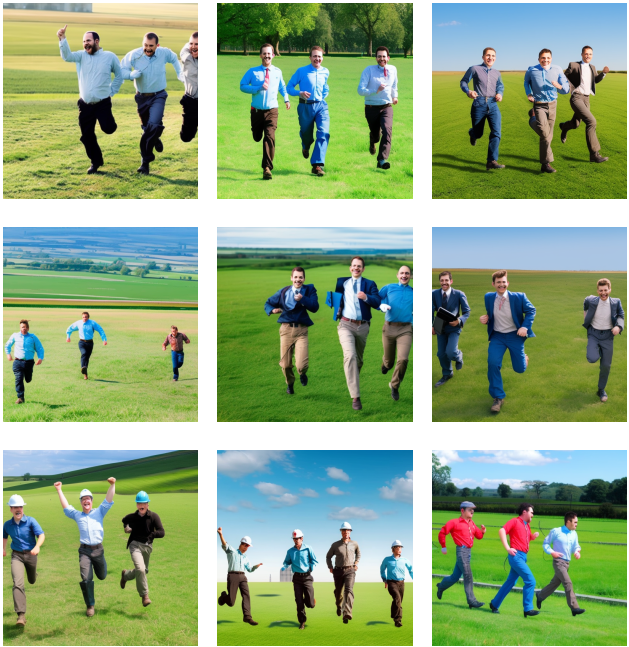
\includegraphics[scale=0.5]{images_generated_with_text_three_engineers.png}
%   \caption{Imagem gerada a partir do texto "Three engineers running on the grassland" by Stable Diffusion v2.1.}
%   \label{fig:images_of_three_engineers}
% \end{figure} 

\begin{wrapfigure}{r}{0.50\textwidth}
  \centering 
  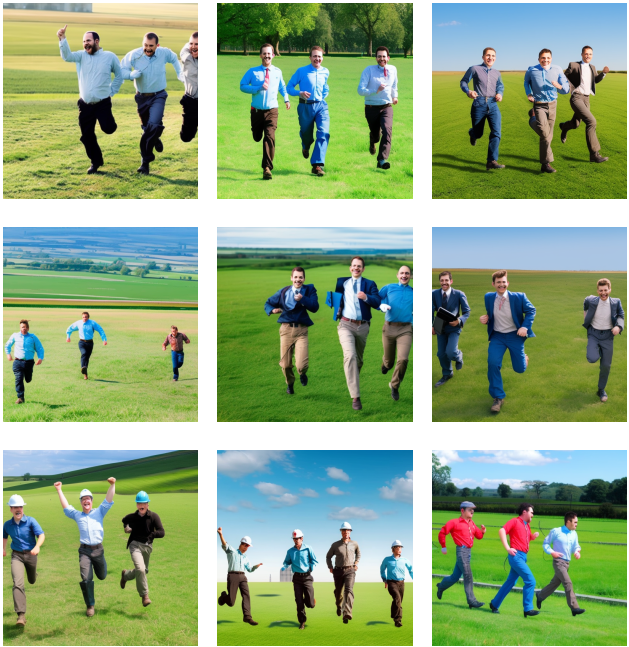
\includegraphics[scale=0.47]{images_generated_with_text_three_engineers.png}
  \caption{Imagem gerada a partir do texto ``Three engineers running on the grassland'' \space  by Stable Diffusion v2.1.}
  \label{fig:images_of_three_engineers}
\end{wrapfigure}


% \begin{wrapfigure}{l}{0.25\textwidth}
%     \centering
%     \includegraphics[width=0.25\textwidth]{contour}
% \end{wrapfigure}

% Considerando questões relativas à proteção da propriedade intelectual, 
A medida que as técnicas avançam surgem situações de violação de direitos autorais
com os conteúdos gerados artificialmente. Um dos desafios é associar a legislação da propriedade intelectual, 
que define de forma clara o que é um trabalho original, 
a quando o direito à propriedade intelectual é violado. Por isso, a definição de propriedade intelectual no âmbito 
dos modelos de geração de conteúdos por IA permanece obscura e indefinida.
Alguns exemplos de problemas surgem em modelos geradores 
baseados em texto-para-imagem, acusados de infringir os trabalhos de artistas plásticos \textbf{(será que não seria apenas artistas?)}, 
consequência do uso de grandes volumes de imagens da internet para o treinamento dos modelos como Stable Diffusion.
% Acho que o Copilot não é treinado em imagens





Uma estratégia de minimizar a violação da propriedade intelectual é permitir que os artistas que considerarem seus direitos autorais
violados tenham seus trabalhos removidos dos datasets, como a empresa Midjourney. 
Outras companhias, como Stability AI, planejam permitir que os próprios artistas removam seus trabalhos, 
dando mais flexibilidade ao processo de proteção intelectual. 
Para textos, a marca d'água têm sido utilizada auxiliando na verificação do uso de fontes sem permissão para a geração 
de conteúdos. A companhia OpenAI trabalha para disponibilizar um classificador que consiga diferenciar entre 
texto gerado por modelos de IA e textos escritos por pessoas.


Após breve análise dos principais elementos desejáveis no escopo de GCIA responsáveis, faz-se necessário avaliar  
outras característivas que devem existir nos modelos.

Assim, os conteúdos gerados pelos modelos GCIA podem propagar informação oculta, violenta, danosa e falsa, onde os textos e 
imagens são difíceis de serem diferenciadas de conteúdos criados por pessoas, e podem ser utilizados para propósitos 
de publicação de notícias falsas (\textit{fake news}), boatos e até mensagens de assédio. 
Além disso, o uso para fins comerciais de imagens e textos inseridos 
em produtos e soluções, a integração dos modelos em software e sistemas, a possibiidade da substituição 
de determinados trabalhos realizados por pessoas de uma forma descontrolada gera bastante controversia.

Os modelos podem ser vistos como caixas-preta tendo uma entrada, o processamento que é oculto aos olhos dos usuários 
e a saída, o que leva a uma necessidade de se explicar esse resultado a fim de se compreender como e por quê foi criado.
Adicionalmente a disponibilidade de código-fonte aberto desses modelos pode resultar em riscos de se propagar as falhas 
já mencionadas anteriormente nos novos modelos, produzindo impactos imprevisíveis. 
A possibilidade dos usuários fornecerem devolutivas \textit{feedback} sobre o uso dos modelos é algo necessário
para se ter modelos responsáveis. Como exemplo, a OpenAI possibilita que usuários enviem feedback
os quais são utilizados para a correção e melhoria reduzindo possíveis impactos negativos.

Outro ponto relevante é que os modelos são treinados com dados sem o devido consentimento, desrespeitando os direitos
autorais e sem compensação aos autores pelo uso dos dados. Para evitar esse problema, as companhias passsaram 
a agir de forma ativa junto aos proprietários dos dados antes de realizarem o treinamento de seus modelos. 
Um caminho para contornar essa situação seria as empresas procurarem os autores solicitando autorização 
para uso dos dados bem como recompensá-los quando os dados forem consultados. Com isso haveria uma justa contrapartida 
para os autores e o uso responsável dos dados pelos modelos.

Outros impactos de dimensões menores, contudo não menos importante é o elevado consumo de energia elétrica pelos computadores a fim de treinar os modelos 
cada vez maiores podendo ter bilhões ou trilhões de parâmetros. Isso leva a uma nova reflexão ainda sem uma solução 
concreta. Adicionalmente os modelos deveriam buscar o equilíbrio de benefícios onde determinados grupos de 
pessoas podem ser privilegiadas em detrimento de outros grupos resultando em desigualdades globais.

Por fim, observa-se nos modelos de GCIA a existencia de conflitos entre seus diversos objetivos, pois ao focar na prevenção 
de determinado risco pode-se criar uma vulnerabilidade em outro tipo de risco. Um exemplo seria quando se busca mitigar 
o uso de termos tóxicos em modelos de linguagem podem surgir viéses na predição que discrimina outras 
comunidades.

O artigo finaliza indicando que GCIA ainda está em uma fase embrionária, em crescente e rápida eovlução, 
com tecnologias impressionantes relacionadas ao campo das artes, mas com vários riscos inerentes ao seu uso. 
Fornece um resumo dos atuais e potenciais riscos devido ao uso dos modelos possibilitando que as Companhias
e usuários se previnam, propondo várias ações para minimizar a ocorrência desses riscos.
Conhecê-los, discutí-los, medí-los e agir é um bom caminho para o futuro dos modelos de GCIA responsáveis.
